% \documentclass[11pt,twoside,a4paper]{article}
% \usepackage{times}

% \usepackage{xeCJK}

% \setmainfont{Times New Roman}

% \setCJKmainfont{Songti SC}
\documentclass[10pt]{ctexart}
% \usepackage[UTF-8]{ctex}
\usepackage{amsmath}
\usepackage{amsthm} % 根据 amsthm 的手册, amsthm 的加载要在 amsmath 之后
\usepackage{amssymb}  %为了能使用\mathbb{H} 
\usepackage{booktabs}
\usepackage{multirow}
\usepackage{tabularx}
\usepackage{xcolor}
\usepackage[colorlinks,linkcolor=blue]{hyperref} % 使用超链接
\usepackage{pdfpages}
\usepackage{geometry}
\geometry{a4paper,scale=0.8}
\usepackage{graphicx} %插入图片的宏包
\usepackage{float} %设置图片浮动位置的宏包
\usepackage{subfigure} %插入多图时用子图显示的宏包
\usepackage{graphicx}

\newtheorem{definition}{定义}
\newtheorem{lemma}{引理}
\newtheorem{theorem}{定理}



\title{零知识证明笔记}
\author{谢文进}
\date{\today}
\begin{document}
\maketitle
\tableofcontents

\section{TO-DO}
\begin{itemize}
	\item 线性变换
	\item 不可约多项式
\end{itemize}

\section{基本概念}
\subsection{抽象代数}
参考资料
\begin{itemize}
	\item 《抽象代数》张贤科 { } 清华大学出版社
	\item 《高等代数》(第三版)北京大学数学系几何与代数教研室
\end{itemize}

\begin{theorem}[古典代数学基本定理]
	任意$n$次方程$x^n+a_1x^{n-1}+ \cdots + a_{n-1}x + a_n = 0$一定有复数解(这里$a_1, \cdots, a_n$为任意复数,整数$n \ge 1$).
\end{theorem}

一个\textbf{集合}就是一些互异的确定的对象全体,其中每个对象称为一个成员或元素,简称为元,有时也称为点。

\textbf{映射三要素}:定义域、值域、对应规则。对任意两个不同的原像,它们有不同的像,则为\textbf{单射}。

以$(a,b)$或gcd$(a,b)$记$a,b$的正的最大公因子。
\begin{lemma}\label{lemma:abqr}
	若$a=bq+r$,其中$a,b,r$为整数(不全为0),则
	$$
	(a,b)=(r,b).
	$$
\end{lemma}
《高等代数》中有类似引理。
\begin{lemma}[《高等代数》P13]
	如果有等式
	\begin{equation}
		f(x) = q(x)g(x)+r(x)
	\end{equation}
	成立,那么$f(x),g(x)$和$g(x),r(x)$有相同的公因式。
\end{lemma}

引理\ref{lemma:abqr}中的公式$(a,b)=(r,b)$说明:余数$r$可作为原数$a$的“替身”去参与求最大公因子,以此类推,引出著名的\textbf{“辗转相除法”}。

\begin{theorem}
	任意两个整数$a,b(b \neq 0)$的最大公因子$d = (a,b)$是唯一存在的,即$d = r_s$(就是$a$与$b$辗转相除的最后非零余数),而且存在整数$u,v$使
	$$
	ua + vb = d \quad(\textbf{贝祖等式},\text{B\'ezout's identity}).
	$$
\end{theorem}

\begin{definition}[《抽象代数》张贤科P17]
	一个\textbf{群}就是一个非空集合$G$,且其元素之间有一种运算,此运算将$G$中任意元素$a$,$b$(可以相等)对应于$G$中的一个元素(记为$a \cdot b$或$ab$),而且满足如下4个条件(称为\textbf{群的公理}):
	\begin{enumerate}
		\item[(G1)](封闭性)$ab$仍然在$G$中(对任意$a$,$b \in G$);
		\item[(G2)](结合律)$a(bc)=(ab)c$(对任意$a,b,c \in G$);
		\item[(G3)](存在单位元)存在元素$e \in G$使$ea = ae = a$(对任意$a \in G$);
		\item[(G4)](可逆性)对每个元素$a \in G$,存在$a' \in G$使$a'a = a a' = e$.
	\end{enumerate}
\end{definition}
满足交换律的群称为\textbf{交换群},或\textbf{Abel群}。

由一个元素$a$生成的子群,称为\textbf{循环子群},记为$\langle a \rangle $.如果群$G=\langle a \rangle$,则$G$称为\textbf{循环群}.


\begin{theorem}[算术基本定理,参考维基百科]
	算术基本定理,又称为正整数的唯一分解定理,即:每个大于1的自然数,要么本身就是质数,要么可以写为2个或以上的质数的积,而且这些质因子按大小排列之后,写法仅有一种方式。
\end{theorem}

\textbf{充分条件与必要条件}
\begin{itemize}
	\item 由条件能推出结论,但由结论推不出这个条件,这个条件就是充分条件。
	\item 如果能由结论推出条件,但由条件推不出结论,此条件为必要条件。
	\item 如果既能由结论推出条件,又能有条件推出结论,此条件为充要条件。
\end{itemize}

\subsection{初等数论}
\subsubsection{原根}
参考\href{https://oi-wiki.org/math/number-theory/primitive-root/#%E5%8E%9F%E6%A0%B9}{oi-wiki原根},一些数学概念及定理如下:
\begin{definition}
	\textbf{阶}:由欧拉定理可知,对 $a\in \mathbb{Z}$,$m\in\mathbb{N}^{*}$,若 $\gcd(a,m)=1$,则 $a^{\varphi(m)}\equiv 1\pmod m$。
	因此满足同余式 $a^n \equiv 1 \pmod m$ 的最小正整数 $n$ 存在,这个 $n$ 称作 $a$ 模 $m$ 的阶,记作 $\delta_m(a)$。
\end{definition}

\begin{definition}
	\textbf{原根}:设 $m \in \mathbb{N}^{*}$,$a\in \mathbb{Z}$。若 $\gcd(a,m)=1$,且 $\delta_m(a)=\varphi(m)$,则称 $a$ 为模 $m$ 的原根。
\end{definition}

\begin{theorem}[原根判定定理]
	设 $m \geqslant 3$, $\gcd(a,m)=1$,则 $a$ 是模 $m$ 的原根的充要条件是,对于 $\varphi(m)$ 的每个素因数 $p$,都有 $a^{\frac{\varphi(m)}{p}}\not\equiv 1\pmod m$。
\end{theorem}
\begin{proof}
	必要性显然,下面用反证法证明充分性。

	当对于 $\varphi(m)$ 的每个素因数 $p$,都有$a^{\frac{\varphi(m)}{p}}\not\equiv 1\pmod m$ 成立时,我们假设存在一个 $a$,其不是模 $m$ 的原根。
	因为 $a$ 不是 $m$ 的原根,则存在一个 $t<\varphi(m)$ 使得 $a^t\equiv 1\pmod{m}$。

	由 裴蜀定理 得,一定存在一组 $k,x$ 满足 $kt=x\varphi(m)+\gcd(t,\varphi(m))$。
	又由 欧拉定理 得 $a^{\varphi(m)}\equiv 1\pmod{m}$,故有:
	$$
	1\equiv a^{kt}\equiv a^{x\varphi(m)+\gcd(t,\varphi(m))}\equiv a^{\gcd(t,\varphi(m))}\pmod{m}
	$$
	由于 $\gcd(t, \varphi(m)) \mid \varphi(m)$ 且 $\gcd(t, \varphi(m))\leqslant t < \varphi(m)$。
	故存在 $\varphi(m)$ 的素因数 $p$ 使得 
	$$ 
	\gcd(t, \varphi(m)) \mid \frac{\varphi(m)}{p}。
	$$
	则$a^{\frac{\varphi(m)}{p}}\equiv a^{(t, \varphi(m))}\equiv 1\pmod{m}$,与条件矛盾。

	故假设不成立,原命题成立。
\end{proof}

\begin{theorem}[原根存在定理]
	一个数 m 存在原根当且仅当 $m=2,4,p^{\alpha},2p^{\alpha}$,其中 $p$ 为奇素数,$\alpha\in \mathbb{N}^{*}$。
\end{theorem}

\subsection{计算复杂度}
参考\href{https://zh.wikipedia.org/wiki/P/NP%E9%97%AE%E9%A2%98}{P/NP问题}、\href{https://zh.wikipedia.org/wiki/NP%E5%AE%8C%E5%85%A8}{NP完全}、\href{https://zhuanlan.zhihu.com/p/73953567}{P问题、NP问题、NP完全问题和NP难问题}:
\begin{itemize}
	\item \textbf{P问题}:复杂度类P即为所有可以由一个确定型图灵机在多项式表达的时间内解决的问题。
	\item \textbf{NP问题}:类NP由所有可以在多项式时间内验证它的解是否正确的决定问题组成,或者等效的说,那些可以在非确定型图灵机上在多项式时间内找出解的问题的集合。
	\item \textbf{NPC问题}:一个决定性问题$C$若是为NPC(NP完全),则代表它对NP是完全的,这表示:
	\begin{itemize}
		\item 它是一个NP问题
		\item 它是一个NP困难问题
		\item 其他属于NP的问题都可在多项式时间内归约(reduce to)成它。
	\end{itemize}
	可归约(reducible)在此意指对每个问题$L$,总有一个多项式时间多对一变换,即一个决定性的算法可以将实例 $l \in L$ 转化成实例 $c \in C$ ,并让$c$回答Yes当且仅当此答案对$l$也是Yes。为了证明某个NP问题A实际上是NP完全问题,证明者必须找出一个已知的NP完全问题可以归约成A。

	\item \textbf{NP难问题}:NP-Hard问题是这样一种问题,它满足NPC问题定义的第二条但不一定要满足第一条(就是说,NP-Hard问题要比 NPC问题的范围广,NP-Hard问题没有限定属于NP),即所有的NP问题都能约化到它,但是它不一定是一个NP问题。
\end{itemize}
它们之间的关系如下:
\begin{figure}[H]
    \centering
    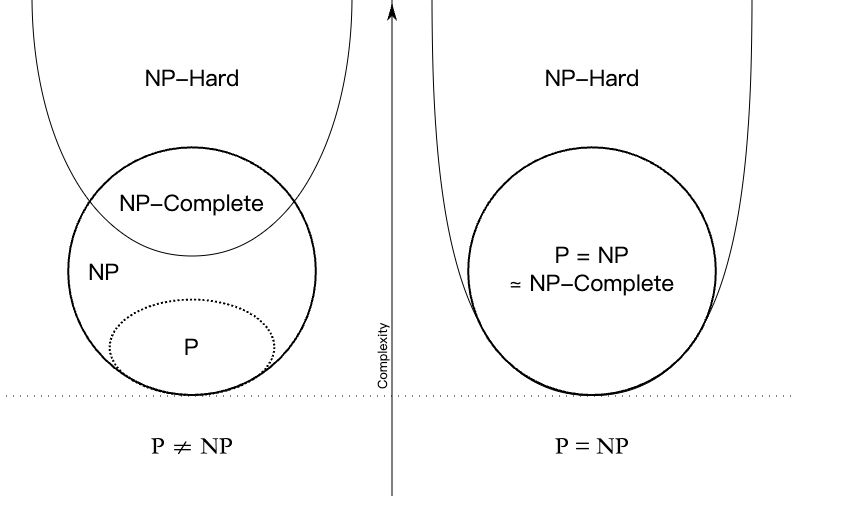
\includegraphics[width=0.6\textwidth]{./img/p_np_npc_nph.png} 
\end{figure}
\subsection{密码学基础}
参考课程\href{https://www.bilibili.com/video/BV18T411k74f/?spm_id_from=333.788&vd_source=c6586ed2410fae637f393017e00f4845}{密码学系列讲座}。
\subsection{区块链技术}
参考课程\href{http://zhenxiao.com/blockchain/}{区块链技术与应用}。
\section{零知识证明}
% \subsection{交互式零知识证明}
% 参考课程\href{https://zk-learning.org/}{Zero Knowledge Proofs}。
% \begin{definition}
% 	A language $\mathcal{L}$ is a set of binary strings $x$.
% \end{definition}
% \begin{definition}
% 	$\mathcal{L}$ is an \textbf{NP}-language (or NP-decision problem), if there is a \textbf{poly$(|x|)$ time} verify $V$ where
% 	\begin{itemize}
% 		 \item \textbf{Completeness [True claims have (short) proofs].}
		 
% 		if $x \in \mathcal{L}$,there is a poly$(|x|)$-long witness $w \in \{0,1\}^*$ s.t. $V(x,w) = 1.$
% 		\item \textbf{Soundness [False theorems have no proofs].}
		
% 		if $x \notin \mathcal{L}$, there is no witness. That is, for all $w \in \{0,1\}^*,V(x,w) = 0.$
% 	\end{itemize}
% \end{definition}

% \begin{definition}
% 	$(P, V)$ is an interactive proof for L, if V is probabilistic poly $(|x|)$ time and
% 	\begin{itemize}
% 		\item Completeness: If $x \in L$, V always accepts.
% 		\item Soundness: If $x \notin L$, for all {\color{blue}cheating prover strategy}, V will not accept
% 		except with negligible probability.
% 	\end{itemize}
% \end{definition}

% \begin{definition}
% 	$(P, V)$ is an interactive proof for L, if V is probabilistic poly $(|x|)$ and
% 	\begin{itemize}
% 		\item Completeness: If $x\in L$, $Pr[(P,V)(x)= accept]=1$.
% 		\item Soundness: If $x \notin L$, for every $P^*$, $Pr[(P^*,V)(x)= accept]=negl(|x|)$
% 		where $negl(\lambda) \le \frac{1}{polynomial(\lambda)}$ for all polynomial functions.
% 	\end{itemize}
% \end{definition}

% \begin{definition}
% 	$(P, V)$ is an interactive proof for L, if V is probabilistic poly $(|x|)$ and 
% 	\begin{itemize}
% 		\item Completeness: If $x\in L$, $Pr[(P,V)(x)= accept] \ge c$
% 		\item Soundness: If $x \notin L$, for every $P^*$, $Pr[(P^*,V)(x)= accept] \le s$
% 	\end{itemize}
% 	Equivalent as long as $ c-s \ge 1/poly(|x|)$.
% \end{definition}

% \begin{definition}
% 	class of languages IP =
% \{L for which there is an interactive proof\}.
% \end{definition}

% \begin{definition}
% 	An Interactive Protocol $(P,V)$ is \textbf{zero-knowledge} for a language L if there exists a PPT algorithm Sim (a simulator) such that for every $x \in L$, the following two probability distributions are poly-time indistinguishable:
% 	\begin{enumerate}
% 		\item $view_V(P,V)[x, 1^\lambda]$
% 		\item $Sim(x, 1^\lambda)$
% 	\end{enumerate}
% \end{definition}
% \begin{definition}
% 	$(P,V)$ is a \textbf{zero-knowledge interactive protocol} if it is complete, sound and zero-knowledge.
% \end{definition}

% \begin{definition}
% 	An Interactive Protocol $(P,V)$ is zero-knowledge for a language L if for every PPT $V^*$, there exists a poly time simulator Sim s.t. for every $x \in L$,
% 	$$
% 	view_V(P,V)[x] \approx Sim(x,1^\lambda)
% 	$$
% \end{definition}

% \textbf{Flavors of Zero Knowledge}
% \begin{itemize}
% 	\item Computationally indistinguishable distributions = CZK
% 	\item Perfectly identical distributions = PZK
% 	\item Statistically close distributions = SZK
% \end{itemize}

% Consider $L_R=\{x: \exists w \text{ s.t. }  R(x,w)= accept \}$ for poly-time relation $R$.
% \begin{definition}
% 	$(P,V)$ is a \textbf{proof of knowledge} (POK) for $L_R$ if :
% 	$\exists$ PPT (knowledge) extractor algorithm E s. t. $\forall x$ in L,
% 	in expected poly-time $E^P(x)$ outputs w s.t. R(x,w)=accept. {\color{blue}[if $Prob[(P,V)(x)=accept] > \alpha$, then $E^P(x)$ runs in expected poly$(|x|,1/ \alpha)$ time]}
% \end{definition}

% \begin{theorem}[GMW86,Naor]
% 	If one-way functions exist, then every L in NP has \textbf{computational zero knowledge interactive proofs}.
% \end{theorem}

% Properties of a Bit Commitment Protocol (Commit, Decommit) between Sender S and Receiver R
% \begin{itemize}
% 	\item \textbf{Hiding}: $\forall$ receiver $R^*$ , after {\color{blue} commit} stage $\forall b, b' \in {0,1}$, view of sender $R^*$ $\{ View_{R^*}(Sender(b),R^*)(1^k)\}$ $ \approx_c  \{ View_{R^*}(Sender(b'),R^*)(1^k)\}$ [k = sec.param]
% 	\item \textbf{Binding}: $\forall$ sender $S^*$, after {\color{blue} commit} and {\color{blue} decommit stage}, Prob[R will accept two different values b and b’] < negl(k), K-security parameter
% \end{itemize}

% \textbf{Protocol design applications}

% Generally: A tool to enforce honest behavior {\color{violet}in protocols} without revealing any information. Idea: protocol players sends along with each next-msg, a ZK proof that next-msg= Protocol(history h, randomness r) on history h and c=commit(r) Possible since {\color{violet}$L=\{\exists r \text{ s.t. next-msg = Protocol}(h.r) \text{ and } c = commit(r)\}$} in NP.

% \textbf{Arthur-Merlin Games [BaM85]}
% \begin{theorem}[GoldwasserSipser86]
% 	AM (protocols with Public Coins) = IP
% \end{theorem}
% AM Protocols enable "in practice" removal of interaction: the Fiat-Shamir Paradigm[FS87].
% Fiat-Shamir Heuristic:
% If H is random-oracle, then completeness and soundness hold.

% Warning: this does \textbf{NOT} mean every interactive ZK proof can transform to AM
% protocols and then use Fiat-Shamir heuristic, since IP = AM transformation requires extra super-polynomial powers from Merlin. And for Fiat-Shamir heuristic to work, Prover must be computationally bounded so not to be able to invert H. Yet, many specific protocols, can benefit from this heuristic.

% \subsection{Modern SNARKs}
% 参考\href{https://www.youtube.com/watch?v=bGEXYpt3sj0}{ZKP MOOC Lecture 2: Overview of Modern SNARK Constructions}。

% \subsubsection{arithmetic circuits}
% 对于一些素数$p \ge 2$,选定一个有限域$\mathbb{F} = \{0, \cdots, p-1\}$。算术电路:$C: \mathbb{F}^n \rightarrow \mathbb{F}$
% \begin{itemize}
% 	\item 一个有向无环图,其中用$1,x_1,\cdots,x_n$作为输入,内部节点之间有$+,-,\times$运算。
% 	\item 算术电路定义了一个$n$变量的多项式的估计。
% \end{itemize}
% 记$|C| =$ \#gates in $C$,就是电路门数目。
% \begin{figure}[H]
%     \centering
%     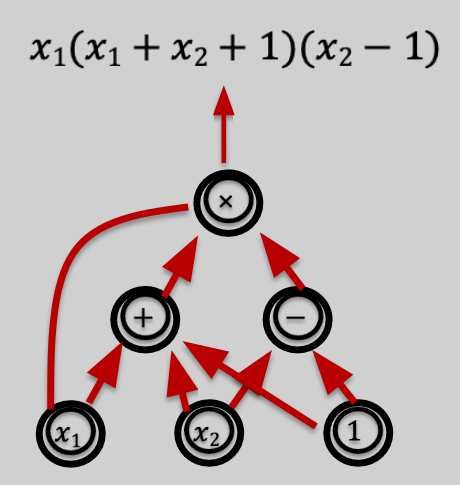
\includegraphics[width=0.4\textwidth]{./img/arithmetic_circuit.png} 
% \end{figure}
% 文章\href{https://secbit.io/blog/2019/07/31/zero-knowledge-and-proof/}{初识「零知识」与「证明」}中说明了可验证计算与电路可满足性问题。所谓的\textbf{电路可满足性}就是指,存在满足电路的一个解。如果这个解的输出值等于一个确定值,那么这个解就能「表示」电路的计算过程。\textbf{零知识的电路可满足性证明协议}提供了一种最直接的保护隐私/敏感数据的技术。

% \textbf{Structured vs. unstructured circuits}

% An unstructured circuit: a circuit with aribitary wires.

% A structured circuit:
% \begin{figure}[H]
%     \centering
%     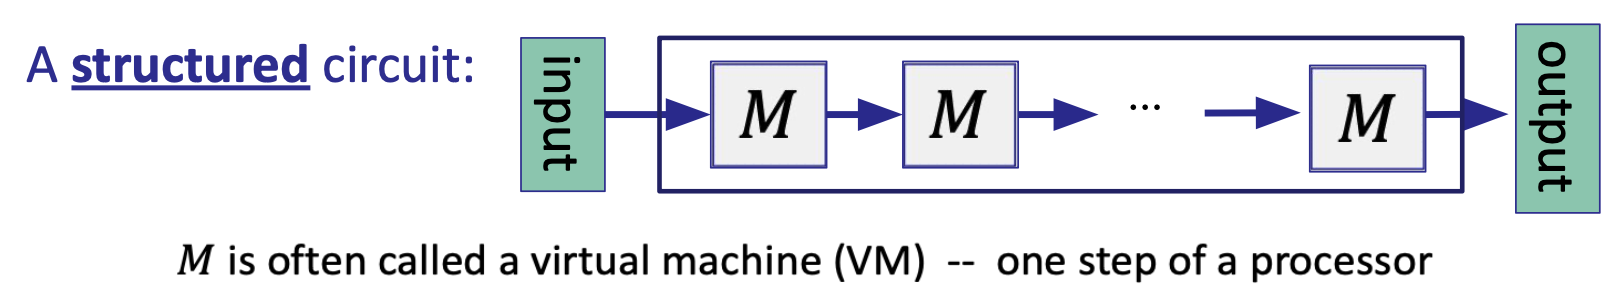
\includegraphics[width=0.9\textwidth]{./img/structured_circuit.png} 
% \end{figure}

% \subsubsection{NARK}
% NARK: Non-interactive ARgument of Knowledge

% 对于公开的算术电路:$C(x,w) \rightarrow \mathbb{F}$,其中$x$是$\mathbb{F}$中公开的陈述(statement),$w$是$\mathbb{F}^m$中的秘密(secret witness)。预处理过程(setup)是:$S(c) \rightarrow (pp,vp)$。
% \begin{figure}[H]
%     \centering
%     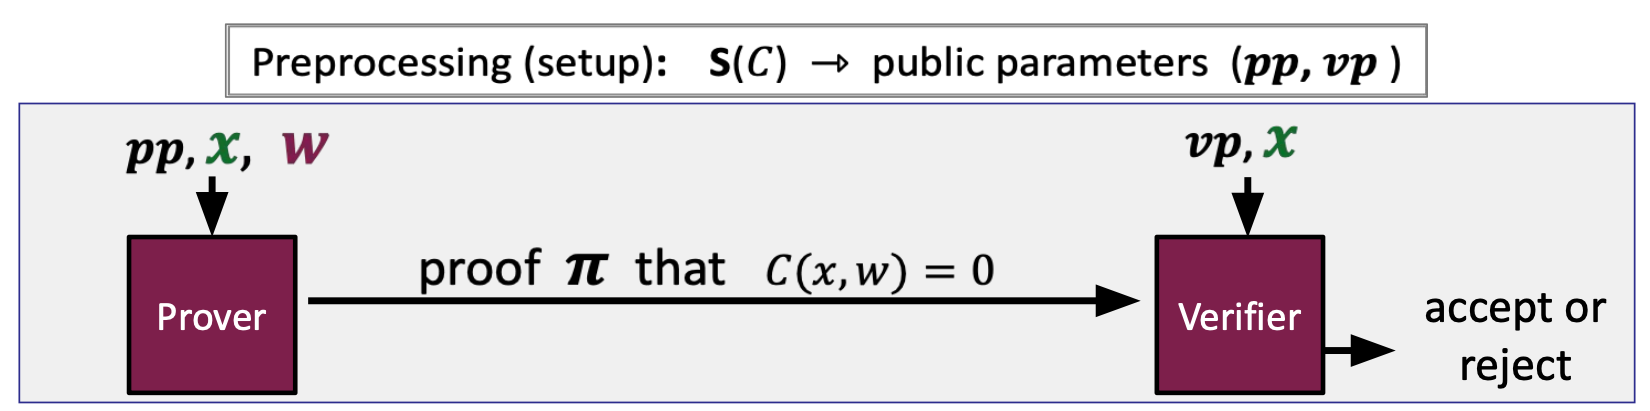
\includegraphics[width=0.9\textwidth]{./img/preprocessing.png} 
% \end{figure}
% 一个预处理的NARK是一个三元组$(S,P,V)$:
% \begin{itemize}
% 	\item $S(C) \rightarrow$ prover和verifier的公开参数$(pp,vp)$
% 	\item $P(pp,x,w) \rightarrow$ 证明 $\pi$
% 	\item $V(vp,x,\pi) \rightarrow$ 接受或拒绝
% \end{itemize}

% NARK中要求:
% \begin{itemize}
% 	\item \textbf{Complete}: $\forall x,w: C(x,w) = 0 \Rightarrow Pr[V(vp,x,P(pp,x,w))=accept] =1$
% 	\item Adaptively \textbf{knowledge sound}: V accepts $\Rightarrow$ P "knows" $w$ s.t. $C(x,w)=0$ (存在一个知识提取器能从$P$中提取出有效的$w$)
% 	\item 可选: \textbf{Zero knowledge}: $(C,pp,vp,x,\pi)$没有泄漏任何关于$w$的新的知识
% \end{itemize}

% \subsubsection*{A succinct preprocessing NARK}
% \begin{figure}[H]
%     \centering
%     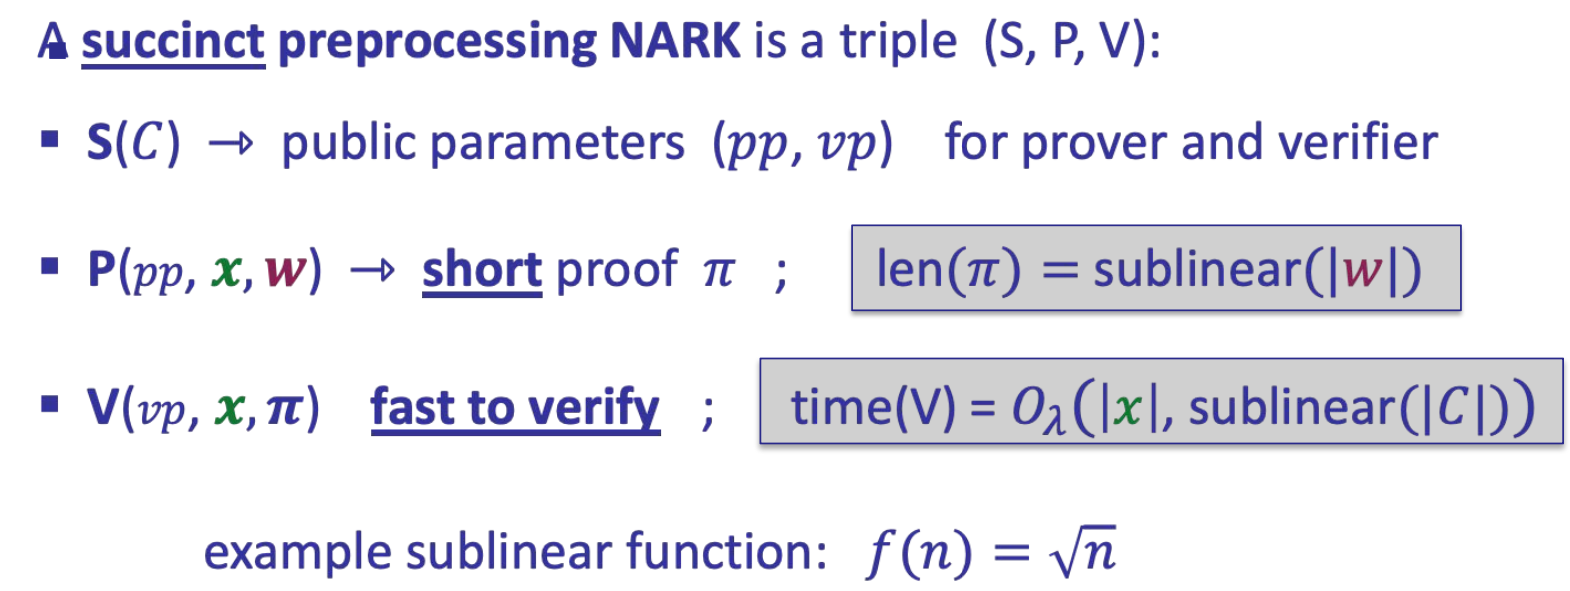
\includegraphics[width=0.9\textwidth]{./img/a_succinct_NARK.png} 
% \end{figure}

% \subsubsection*{A strongly succinct preprocessing NARK}
% \begin{figure}[H]
%     \centering
%     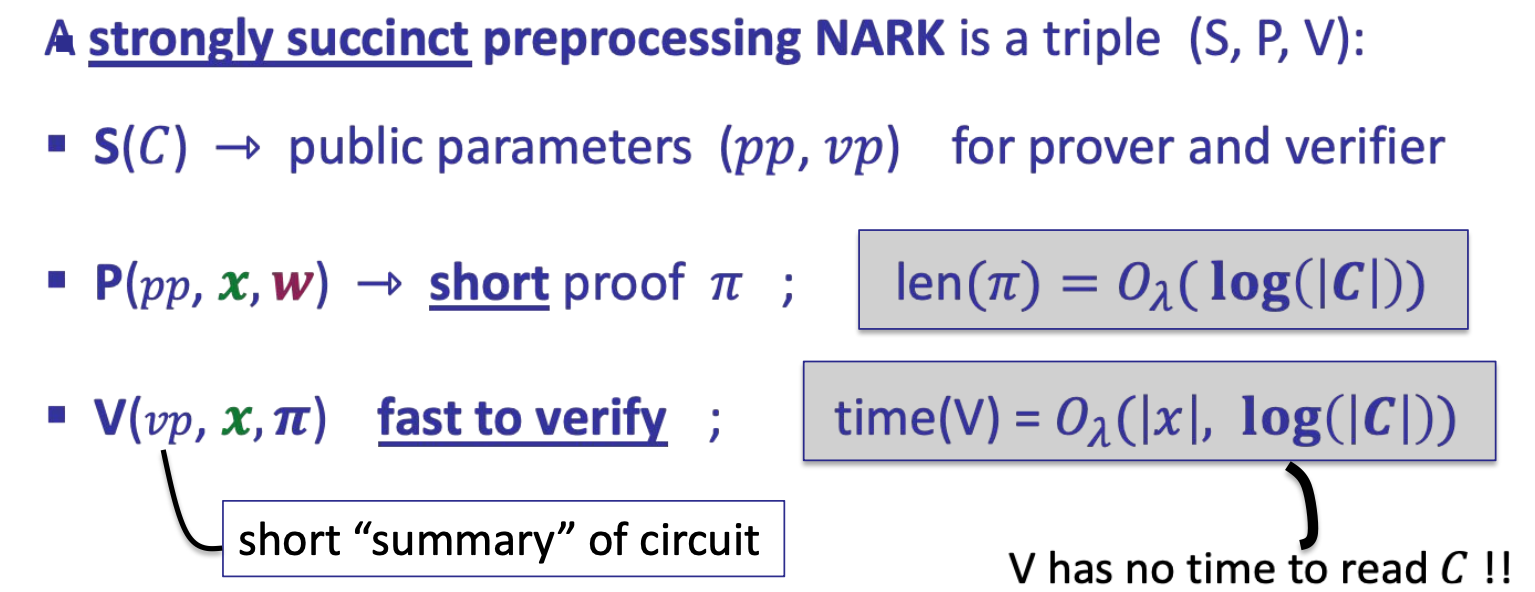
\includegraphics[width=1\textwidth]{./img/a_strongly_succinct_NARK.png} 
% \end{figure}
% SNARK: 就是一个NARK(complete and knowledge sound)是succint.

% zk-SNARK: 就是一个SNARK是zero knowledge.

% \subsubsection*{Types of preprocessing Setup}
% \begin{figure}[H]
%     \centering
%     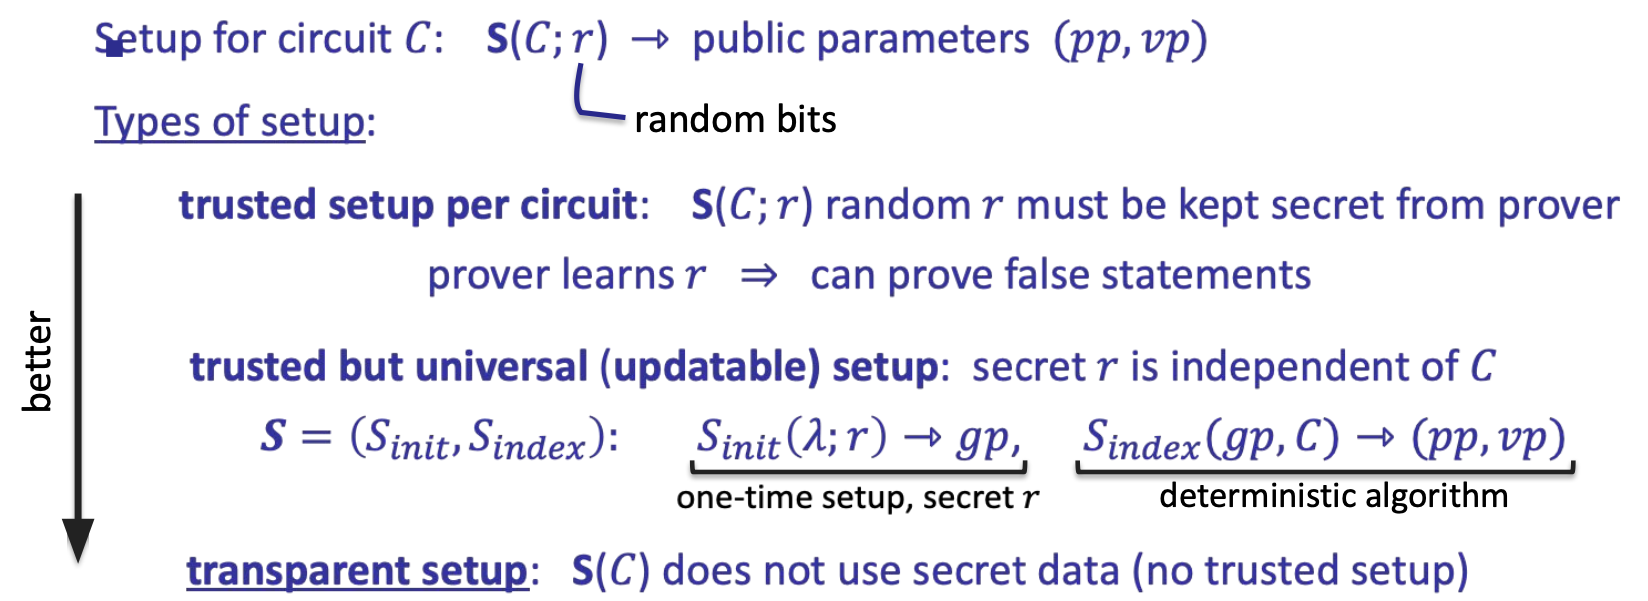
\includegraphics[width=1\textwidth]{./img/types_of_preprocessing_setup.png} 
% \end{figure}

% \subsubsection*{knowledge soundness}

% \begin{figure}[H]
%     \centering
%     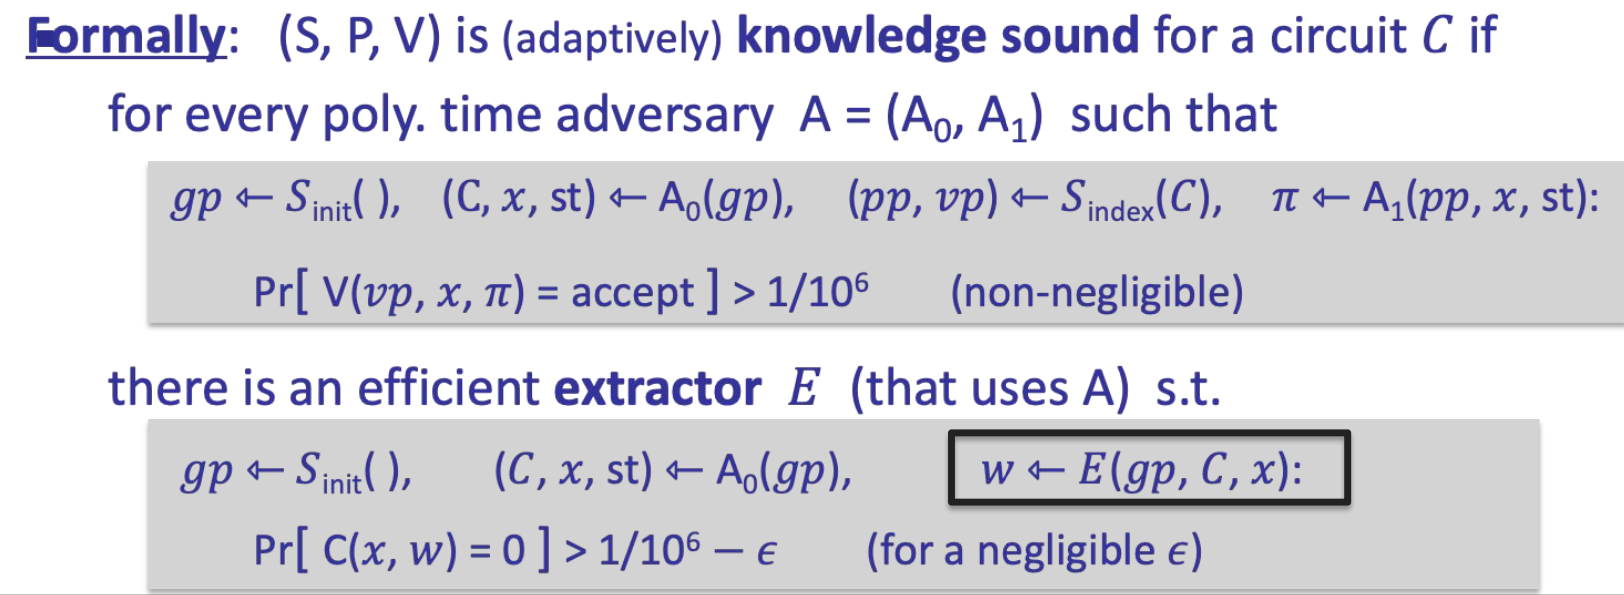
\includegraphics[width=1\textwidth]{./img/knowledge_soundness.png} 
% \end{figure}

% \subsubsection{Building an efficient SNARK}

\end{document}